\documentclass[1p]{elsarticle_modified}
%\bibliographystyle{elsarticle-num}

%\usepackage[colorlinks]{hyperref}
%\usepackage{abbrmath_seonhwa} %\Abb, \Ascr, \Acal ,\Abf, \Afrak
\usepackage{amsfonts}
\usepackage{amssymb}
\usepackage{amsmath}
\usepackage{amsthm}
\usepackage{scalefnt}
\usepackage{amsbsy}
\usepackage{kotex}
\usepackage{caption}
\usepackage{subfig}
\usepackage{color}
\usepackage{graphicx}
\usepackage{xcolor} %% white, black, red, green, blue, cyan, magenta, yellow
\usepackage{float}
\usepackage{setspace}
\usepackage{hyperref}

\usepackage{tikz}
\usetikzlibrary{arrows}

\usepackage{multirow}
\usepackage{array} % fixed length table
\usepackage{hhline}

%%%%%%%%%%%%%%%%%%%%%
\makeatletter
\renewcommand*\env@matrix[1][\arraystretch]{%
	\edef\arraystretch{#1}%
	\hskip -\arraycolsep
	\let\@ifnextchar\new@ifnextchar
	\array{*\c@MaxMatrixCols c}}
\makeatother %https://tex.stackexchange.com/questions/14071/how-can-i-increase-the-line-spacing-in-a-matrix
%%%%%%%%%%%%%%%

\usepackage[normalem]{ulem}

\newcommand{\msout}[1]{\ifmmode\text{\sout{\ensuremath{#1}}}\else\sout{#1}\fi}
%SOURCE: \msout is \stkout macro in https://tex.stackexchange.com/questions/20609/strikeout-in-math-mode

\newcommand{\cancel}[1]{
	\ifmmode
	{\color{red}\msout{#1}}
	\else
	{\color{red}\sout{#1}}
	\fi
}

\newcommand{\add}[1]{
	{\color{blue}\uwave{#1}}
}

\newcommand{\replace}[2]{
	\ifmmode
	{\color{red}\msout{#1}}{\color{blue}\uwave{#2}}
	\else
	{\color{red}\sout{#1}}{\color{blue}\uwave{#2}}
	\fi
}

\newcommand{\Sol}{\mathcal{S}} %segment
\newcommand{\D}{D} %diagram
\newcommand{\A}{\mathcal{A}} %arc


%%%%%%%%%%%%%%%%%%%%%%%%%%%%%5 test

\def\sl{\operatorname{\textup{SL}}(2,\Cbb)}
\def\psl{\operatorname{\textup{PSL}}(2,\Cbb)}
\def\quan{\mkern 1mu \triangleright \mkern 1mu}

\theoremstyle{definition}
\newtheorem{thm}{Theorem}[section]
\newtheorem{prop}[thm]{Proposition}
\newtheorem{lem}[thm]{Lemma}
\newtheorem{ques}[thm]{Question}
\newtheorem{cor}[thm]{Corollary}
\newtheorem{defn}[thm]{Definition}
\newtheorem{exam}[thm]{Example}
\newtheorem{rmk}[thm]{Remark}
\newtheorem{alg}[thm]{Algorithm}

\newcommand{\I}{\sqrt{-1}}
\begin{document}

%\begin{frontmatter}
%
%\title{Boundary parabolic representations of knots up to 8 crossings}
%
%%% Group authors per affiliation:
%\author{Yunhi Cho} 
%\address{Department of Mathematics, University of Seoul, Seoul, Korea}
%\ead{yhcho@uos.ac.kr}
%
%
%\author{Seonhwa Kim} %\fnref{s_kim}}
%\address{Center for Geometry and Physics, Institute for Basic Science, Pohang, 37673, Korea}
%\ead{ryeona17@ibs.re.kr}
%
%\author{Hyuk Kim}
%\address{Department of Mathematical Sciences, Seoul National University, Seoul 08826, Korea}
%\ead{hyukkim@snu.ac.kr}
%
%\author{Seokbeom Yoon}
%\address{Department of Mathematical Sciences, Seoul National University, Seoul, 08826,  Korea}
%\ead{sbyoon15@snu.ac.kr}
%
%\begin{abstract}
%We find all boundary parabolic representation of knots up to 8 crossings.
%
%\end{abstract}
%\begin{keyword}
%    \MSC[2010] 57M25 
%\end{keyword}
%
%\end{frontmatter}

%\linenumbers
%\tableofcontents
%
\newcommand\colored[1]{\textcolor{white}{\rule[-0.35ex]{0.8em}{1.4ex}}\kern-0.8em\color{red} #1}%
%\newcommand\colored[1]{\textcolor{white}{ #1}\kern-2.17ex	\textcolor{white}{ #1}\kern-1.81ex	\textcolor{white}{ #1}\kern-2.15ex\color{red}#1	}

{\Large $\underline{12n_{0053}~(K12n_{0053})}$}

\setlength{\tabcolsep}{10pt}
\renewcommand{\arraystretch}{1.6}
\vspace{1cm}\begin{tabular}{m{100pt}>{\centering\arraybackslash}m{274pt}}
\multirow{5}{120pt}{
	\centering
	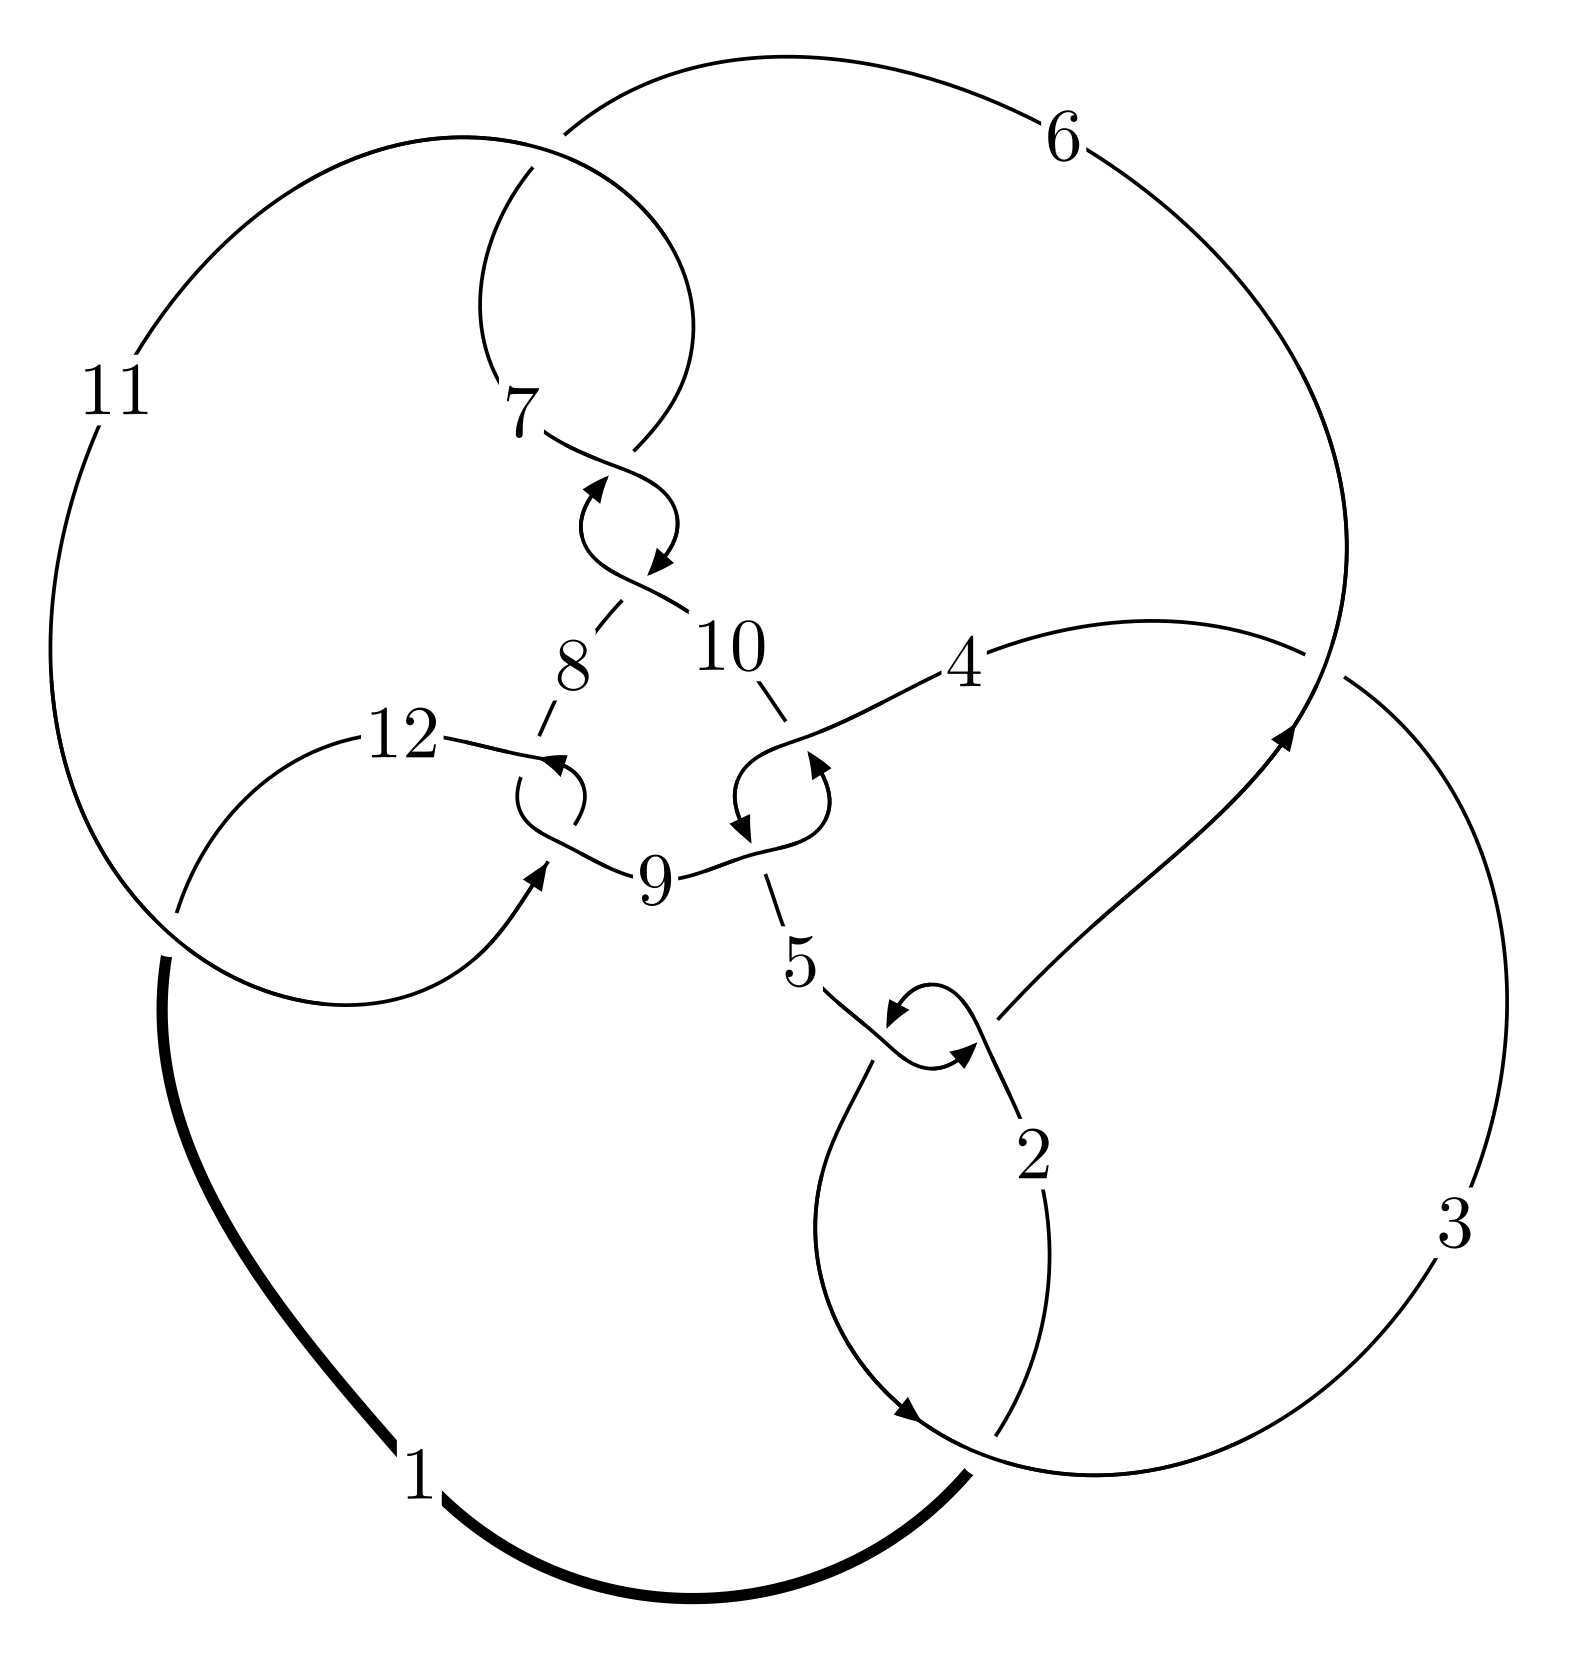
\includegraphics[width=112pt]{../../../GIT/diagram.site/Diagrams/png/2142_12n_0053.png}\\
\ \ \ A knot diagram\footnotemark}&
\allowdisplaybreaks
\textbf{Linearized knot diagam} \\
\cline{2-2}
 &
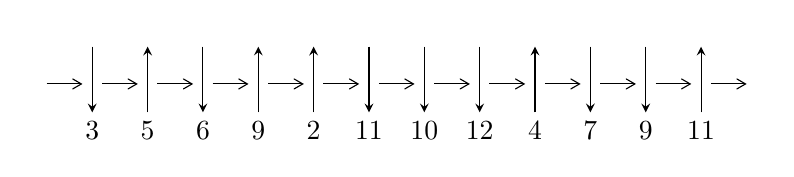
\begin{tikzpicture}[x=20pt, y=17pt]
	% nodes
	\node (C0) at (0, 0) {};
	\node (C1) at (1, 0) {};
	\node (C1U) at (1, +1) {};
	\node (C1D) at (1, -1) {3};

	\node (C2) at (2, 0) {};
	\node (C2U) at (2, +1) {};
	\node (C2D) at (2, -1) {5};

	\node (C3) at (3, 0) {};
	\node (C3U) at (3, +1) {};
	\node (C3D) at (3, -1) {6};

	\node (C4) at (4, 0) {};
	\node (C4U) at (4, +1) {};
	\node (C4D) at (4, -1) {9};

	\node (C5) at (5, 0) {};
	\node (C5U) at (5, +1) {};
	\node (C5D) at (5, -1) {2};

	\node (C6) at (6, 0) {};
	\node (C6U) at (6, +1) {};
	\node (C6D) at (6, -1) {11};

	\node (C7) at (7, 0) {};
	\node (C7U) at (7, +1) {};
	\node (C7D) at (7, -1) {10};

	\node (C8) at (8, 0) {};
	\node (C8U) at (8, +1) {};
	\node (C8D) at (8, -1) {12};

	\node (C9) at (9, 0) {};
	\node (C9U) at (9, +1) {};
	\node (C9D) at (9, -1) {4};

	\node (C10) at (10, 0) {};
	\node (C10U) at (10, +1) {};
	\node (C10D) at (10, -1) {7};

	\node (C11) at (11, 0) {};
	\node (C11U) at (11, +1) {};
	\node (C11D) at (11, -1) {9};

	\node (C12) at (12, 0) {};
	\node (C12U) at (12, +1) {};
	\node (C12D) at (12, -1) {11};
	\node (C13) at (13, 0) {};

	% arrows
	\draw[->,>={angle 60}]
	(C0) edge (C1) (C1) edge (C2) (C2) edge (C3) (C3) edge (C4) (C4) edge (C5) (C5) edge (C6) (C6) edge (C7) (C7) edge (C8) (C8) edge (C9) (C9) edge (C10) (C10) edge (C11) (C11) edge (C12) (C12) edge (C13) ;	\draw[->,>=stealth]
	(C1U) edge (C1D) (C2D) edge (C2U) (C3U) edge (C3D) (C4D) edge (C4U) (C5D) edge (C5U) (C6U) edge (C6D) (C7U) edge (C7D) (C8U) edge (C8D) (C9D) edge (C9U) (C10U) edge (C10D) (C11U) edge (C11D) (C12D) edge (C12U) ;
	\end{tikzpicture} \\
\hhline{~~} \\& 
\textbf{Solving Sequence} \\ \cline{2-2} 
 &
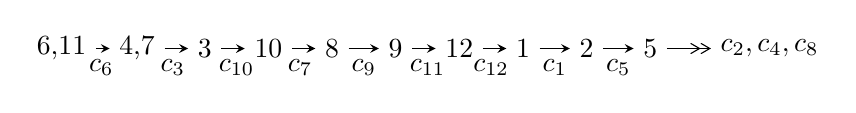
\begin{tikzpicture}[x=23pt, y=7pt]
	% node
	\node (A0) at (-1/8, 0) {6,11};
	\node (A1) at (17/16, 0) {4,7};
	\node (A2) at (17/8, 0) {3};
	\node (A3) at (25/8, 0) {10};
	\node (A4) at (33/8, 0) {8};
	\node (A5) at (41/8, 0) {9};
	\node (A6) at (49/8, 0) {12};
	\node (A7) at (57/8, 0) {1};
	\node (A8) at (65/8, 0) {2};
	\node (A9) at (73/8, 0) {5};
	\node (C1) at (1/2, -1) {$c_{6}$};
	\node (C2) at (13/8, -1) {$c_{3}$};
	\node (C3) at (21/8, -1) {$c_{10}$};
	\node (C4) at (29/8, -1) {$c_{7}$};
	\node (C5) at (37/8, -1) {$c_{9}$};
	\node (C6) at (45/8, -1) {$c_{11}$};
	\node (C7) at (53/8, -1) {$c_{12}$};
	\node (C8) at (61/8, -1) {$c_{1}$};
	\node (C9) at (69/8, -1) {$c_{5}$};
	\node (A10) at (11, 0) {$c_{2},c_{4},c_{8}$};

	% edge
	\draw[->,>=stealth]	
	(A0) edge (A1) (A1) edge (A2) (A2) edge (A3) (A3) edge (A4) (A4) edge (A5) (A5) edge (A6) (A6) edge (A7) (A7) edge (A8) (A8) edge (A9) ;
	\draw[->>,>={angle 60}]	
	(A9) edge (A10);
\end{tikzpicture} \\ 

\end{tabular} \\

\footnotetext{
The image of knot diagram is generated by the software ``\textbf{Draw programme}" developed by Andrew Bartholomew(\url{http://www.layer8.co.uk/maths/draw/index.htm\#Running-draw}), where we modified some parts for our purpose(\url{https://github.com/CATsTAILs/LinksPainter}).
}\phantom \\ \newline 
\centering \textbf{Ideals for irreducible components\footnotemark of $X_{\text{par}}$} 
 
\begin{align*}
I^u_{1}&=\langle 
291 u^{21}-1049 u^{20}+\cdots+2048 b+307,\;1007 u^{21}-2141 u^{20}+\cdots+4096 a-3617,\\
\phantom{I^u_{1}}&\phantom{= \langle  }u^{22}-2 u^{21}+\cdots+11 u^2+1\rangle \\
I^u_{2}&=\langle 
194087126632 u^{17}+1704357838964 u^{16}+\cdots+10770316588487 b+37991651925802,\\
\phantom{I^u_{2}}&\phantom{= \langle  }-107427678939090 u^{17}-569643045714954 u^{16}+\cdots+786233110959551 a-1104507859905079,\\
\phantom{I^u_{2}}&\phantom{= \langle  }u^{18}+5 u^{17}+\cdots+286 u+73\rangle \\
I^u_{3}&=\langle 
- a^4- a^3 u+a^3+2 a^2 u+4 a u+4 b+4 a-4,\;a^5+a^4 u- a^4-2 a^3 u-4 a^2 u-4 a^2+4 a-4 u+4,\;u^2+1\rangle \\
I^u_{4}&=\langle 
b-2 a,\;4 a^2+2 a+1,\;u-1\rangle \\
\\
\end{align*}
\raggedright * 4 irreducible components of $\dim_{\mathbb{C}}=0$, with total 52 representations.\\
\footnotetext{All coefficients of polynomials are rational numbers. But the coefficients are sometimes approximated in decimal forms when there is not enough margin.}
\newpage
\renewcommand{\arraystretch}{1}
\centering \section*{I. $I^u_{1}= \langle 291 u^{21}-1049 u^{20}+\cdots+2048 b+307,\;1007 u^{21}-2141 u^{20}+\cdots+4096 a-3617,\;u^{22}-2 u^{21}+\cdots+11 u^2+1 \rangle$}
\flushleft \textbf{(i) Arc colorings}\\
\begin{tabular}{m{7pt} m{180pt} m{7pt} m{180pt} }
\flushright $a_{6}=$&$\begin{pmatrix}1\\0\end{pmatrix}$ \\
\flushright $a_{11}=$&$\begin{pmatrix}0\\u\end{pmatrix}$ \\
\flushright $a_{4}=$&$\begin{pmatrix}-0.245850 u^{21}+0.522705 u^{20}+\cdots+0.581787 u+0.883057\\-0.142090 u^{21}+0.512207 u^{20}+\cdots-0.498535 u-0.149902\end{pmatrix}$ \\
\flushright $a_{7}=$&$\begin{pmatrix}1\\u^2\end{pmatrix}$ \\
\flushright $a_{3}=$&$\begin{pmatrix}-0.387939 u^{21}+1.03491 u^{20}+\cdots+0.0832520 u+0.733154\\-0.142090 u^{21}+0.512207 u^{20}+\cdots-0.498535 u-0.149902\end{pmatrix}$ \\
\flushright $a_{10}=$&$\begin{pmatrix}u\\u^3+u\end{pmatrix}$ \\
\flushright $a_{8}=$&$\begin{pmatrix}u^2+1\\u^4+2 u^2\end{pmatrix}$ \\
\flushright $a_{9}=$&$\begin{pmatrix}1\\0.0156250 u^{21}-0.0156250 u^{20}+\cdots+0.0156250 u+0.0156250\end{pmatrix}$ \\
\flushright $a_{12}=$&$\begin{pmatrix}- u\\-0.0156250 u^{21}+0.0468750 u^{20}+\cdots+0.984375 u+0.0156250\end{pmatrix}$ \\
\flushright $a_{1}=$&$\begin{pmatrix}- u\\-0.0156250 u^{21}+0.0468750 u^{20}+\cdots+0.984375 u+0.0156250\end{pmatrix}$ \\
\flushright $a_{2}=$&$\begin{pmatrix}-0.0476074 u^{21}+0.0178223 u^{20}+\cdots-6.07739 u+0.889893\\-0.0629883 u^{21}+0.0327148 u^{20}+\cdots-0.0932617 u-0.125488\end{pmatrix}$ \\
\flushright $a_{5}=$&$\begin{pmatrix}-0.118896 u^{21}+0.344971 u^{20}+\cdots-0.420166 u+0.744385\\-0.435059 u^{21}+0.703613 u^{20}+\cdots-1.04932 u-0.661621\end{pmatrix}$\\&\end{tabular}
\flushleft \textbf{(ii) Obstruction class $= -1$}\\~\\
\flushleft \textbf{(iii) Cusp Shapes $= \frac{16767}{8192} u^{21}-\frac{31037}{8192} u^{20}+\cdots+\frac{76033}{8192} u+\frac{27071}{8192}$}\\~\\
\newpage\renewcommand{\arraystretch}{1}
\flushleft \textbf{(iv) u-Polynomials at the component}\newline \\
\begin{tabular}{m{50pt}|m{274pt}}
Crossings & \hspace{64pt}u-Polynomials at each crossing \\
\hline $$\begin{aligned}c_{1}\end{aligned}$$&$\begin{aligned}
&u^{22}+10 u^{21}+\cdots- u+16
\end{aligned}$\\
\hline $$\begin{aligned}c_{2},c_{5}\end{aligned}$$&$\begin{aligned}
&u^{22}+2 u^{21}+\cdots+15 u+4
\end{aligned}$\\
\hline $$\begin{aligned}c_{3}\end{aligned}$$&$\begin{aligned}
&u^{22}-2 u^{21}+\cdots+663 u+676
\end{aligned}$\\
\hline $$\begin{aligned}c_{4},c_{9}\end{aligned}$$&$\begin{aligned}
&u^{22}+3 u^{21}+\cdots+120 u+32
\end{aligned}$\\
\hline $$\begin{aligned}c_{6},c_{7},c_{8}\\c_{10},c_{11}\end{aligned}$$&$\begin{aligned}
&u^{22}+2 u^{21}+\cdots+11 u^2+1
\end{aligned}$\\
\hline $$\begin{aligned}c_{12}\end{aligned}$$&$\begin{aligned}
&u^{22}-30 u^{21}+\cdots-22 u+1
\end{aligned}$\\
\hline
\end{tabular}\\~\\
\newpage\renewcommand{\arraystretch}{1}
\flushleft \textbf{(v) Riley Polynomials at the component}\newline \\
\begin{tabular}{m{50pt}|m{274pt}}
Crossings & \hspace{64pt}Riley Polynomials at each crossing \\
\hline $$\begin{aligned}c_{1}\end{aligned}$$&$\begin{aligned}
&y^{22}+6 y^{21}+\cdots-1857 y+256
\end{aligned}$\\
\hline $$\begin{aligned}c_{2},c_{5}\end{aligned}$$&$\begin{aligned}
&y^{22}+10 y^{21}+\cdots- y+16
\end{aligned}$\\
\hline $$\begin{aligned}c_{3}\end{aligned}$$&$\begin{aligned}
&y^{22}+2 y^{21}+\cdots+1664143 y+456976
\end{aligned}$\\
\hline $$\begin{aligned}c_{4},c_{9}\end{aligned}$$&$\begin{aligned}
&y^{22}+5 y^{21}+\cdots-1216 y+1024
\end{aligned}$\\
\hline $$\begin{aligned}c_{6},c_{7},c_{8}\\c_{10},c_{11}\end{aligned}$$&$\begin{aligned}
&y^{22}+30 y^{21}+\cdots+22 y+1
\end{aligned}$\\
\hline $$\begin{aligned}c_{12}\end{aligned}$$&$\begin{aligned}
&y^{22}-78 y^{21}+\cdots+102 y+1
\end{aligned}$\\
\hline
\end{tabular}\\~\\
\newpage\flushleft \textbf{(vi) Complex Volumes and Cusp Shapes}
$$\begin{array}{c|c|c}  
\text{Solutions to }I^u_{1}& \I (\text{vol} + \sqrt{-1}CS) & \text{Cusp shape}\\
 \hline 
\begin{aligned}
u &= \phantom{-}0.615782 + 0.803264 I \\
a &= -0.547833 - 0.548126 I \\
b &= \phantom{-}1.219690 - 0.593054 I\end{aligned}
 & -3.37145 + 2.38944 I & -5.45481 - 0.71996 I \\ \hline\begin{aligned}
u &= \phantom{-}0.615782 - 0.803264 I \\
a &= -0.547833 + 0.548126 I \\
b &= \phantom{-}1.219690 + 0.593054 I\end{aligned}
 & -3.37145 - 2.38944 I & -5.45481 + 0.71996 I \\ \hline\begin{aligned}
u &= \phantom{-}1.046550 + 0.353921 I \\
a &= \phantom{-}0.455127 + 0.346832 I \\
b &= \phantom{-}0.134390 + 0.768351 I\end{aligned}
 & -1.70749 - 1.42840 I & -2.82321 - 4.75814 I \\ \hline\begin{aligned}
u &= \phantom{-}1.046550 - 0.353921 I \\
a &= \phantom{-}0.455127 - 0.346832 I \\
b &= \phantom{-}0.134390 - 0.768351 I\end{aligned}
 & -1.70749 + 1.42840 I & -2.82321 + 4.75814 I \\ \hline\begin{aligned}
u &= \phantom{-}0.282269 + 0.708144 I \\
a &= -0.640971 - 0.473149 I \\
b &= \phantom{-}1.246260 + 0.317348 I\end{aligned}
 & -3.66689 - 5.42682 I & -7.22851 + 8.75440 I \\ \hline\begin{aligned}
u &= \phantom{-}0.282269 - 0.708144 I \\
a &= -0.640971 + 0.473149 I \\
b &= \phantom{-}1.246260 - 0.317348 I\end{aligned}
 & -3.66689 + 5.42682 I & -7.22851 - 8.75440 I \\ \hline\begin{aligned}
u &= \phantom{-}0.344516 + 0.519144 I \\
a &= \phantom{-}0.672348 + 0.637144 I \\
b &= -0.738214 - 0.182816 I\end{aligned}
 & -0.71829 - 1.39692 I & -3.45104 + 5.22381 I \\ \hline\begin{aligned}
u &= \phantom{-}0.344516 - 0.519144 I \\
a &= \phantom{-}0.672348 - 0.637144 I \\
b &= -0.738214 + 0.182816 I\end{aligned}
 & -0.71829 + 1.39692 I & -3.45104 - 5.22381 I \\ \hline\begin{aligned}
u &= -0.008200 + 0.342361 I \\
a &= \phantom{-}1.46314 + 0.68949 I \\
b &= -0.072113 - 0.750151 I\end{aligned}
 & \phantom{-}0.55339 - 1.37498 I & \phantom{-}1.51135 + 4.45596 I \\ \hline\begin{aligned}
u &= -0.008200 - 0.342361 I \\
a &= \phantom{-}1.46314 - 0.68949 I \\
b &= -0.072113 + 0.750151 I\end{aligned}
 & \phantom{-}0.55339 + 1.37498 I & \phantom{-}1.51135 - 4.45596 I\\
 \hline 
 \end{array}$$\newpage$$\begin{array}{c|c|c}  
\text{Solutions to }I^u_{1}& \I (\text{vol} + \sqrt{-1}CS) & \text{Cusp shape}\\
 \hline 
\begin{aligned}
u &= -0.21154 + 1.66696 I \\
a &= \phantom{-}0.133816 + 1.107720 I \\
b &= -0.091644 - 1.122210 I\end{aligned}
 & \phantom{-}9.07448 + 4.87395 I & -0.77042 - 2.44706 I \\ \hline\begin{aligned}
u &= -0.21154 - 1.66696 I \\
a &= \phantom{-}0.133816 - 1.107720 I \\
b &= -0.091644 + 1.122210 I\end{aligned}
 & \phantom{-}9.07448 - 4.87395 I & -0.77042 + 2.44706 I \\ \hline\begin{aligned}
u &= -0.221701 + 0.205211 I \\
a &= -2.25437 - 0.26322 I \\
b &= -0.678597 + 0.748849 I\end{aligned}
 & -0.25879 + 2.47978 I & \phantom{-}1.67019 - 4.37089 I \\ \hline\begin{aligned}
u &= -0.221701 - 0.205211 I \\
a &= -2.25437 + 0.26322 I \\
b &= -0.678597 - 0.748849 I\end{aligned}
 & -0.25879 - 2.47978 I & \phantom{-}1.67019 + 4.37089 I \\ \hline\begin{aligned}
u &= \phantom{-}0.10555 + 1.78725 I \\
a &= \phantom{-}0.354067 + 1.025410 I \\
b &= -1.93664 - 1.43012 I\end{aligned}
 & \phantom{-}14.0985 - 4.5775 I & \phantom{-}1.42593 + 2.45051 I \\ \hline\begin{aligned}
u &= \phantom{-}0.10555 - 1.78725 I \\
a &= \phantom{-}0.354067 - 1.025410 I \\
b &= -1.93664 + 1.43012 I\end{aligned}
 & \phantom{-}14.0985 + 4.5775 I & \phantom{-}1.42593 - 2.45051 I \\ \hline\begin{aligned}
u &= -0.50678 + 1.71782 I \\
a &= \phantom{-}0.038804 + 1.316300 I \\
b &= \phantom{-}1.79372 - 1.43052 I\end{aligned}
 & \phantom{-}14.3505 + 13.9596 I & \phantom{-}0.89017 - 6.70291 I \\ \hline\begin{aligned}
u &= -0.50678 - 1.71782 I \\
a &= \phantom{-}0.038804 - 1.316300 I \\
b &= \phantom{-}1.79372 + 1.43052 I\end{aligned}
 & \phantom{-}14.3505 - 13.9596 I & \phantom{-}0.89017 + 6.70291 I \\ \hline\begin{aligned}
u &= -0.41437 + 1.78716 I \\
a &= -0.115876 - 1.281550 I \\
b &= -1.17420 + 1.93112 I\end{aligned}
 & \phantom{-}16.3189 + 7.7022 I & \phantom{-}2.88848 - 2.54222 I \\ \hline\begin{aligned}
u &= -0.41437 - 1.78716 I \\
a &= -0.115876 + 1.281550 I \\
b &= -1.17420 - 1.93112 I\end{aligned}
 & \phantom{-}16.3189 - 7.7022 I & \phantom{-}2.88848 + 2.54222 I\\
 \hline 
 \end{array}$$\newpage$$\begin{array}{c|c|c}  
\text{Solutions to }I^u_{1}& \I (\text{vol} + \sqrt{-1}CS) & \text{Cusp shape}\\
 \hline 
\begin{aligned}
u &= -0.03207 + 1.84087 I \\
a &= -0.308249 - 1.105700 I \\
b &= \phantom{-}1.29737 + 1.95650 I\end{aligned}
 & \phantom{-}16.1897 + 1.7866 I & \phantom{-}3.21686 - 1.63436 I \\ \hline\begin{aligned}
u &= -0.03207 - 1.84087 I \\
a &= -0.308249 + 1.105700 I \\
b &= \phantom{-}1.29737 - 1.95650 I\end{aligned}
 & \phantom{-}16.1897 - 1.7866 I & \phantom{-}3.21686 + 1.63436 I\\
 \hline 
 \end{array}$$\newpage\newpage\renewcommand{\arraystretch}{1}
\centering \section*{II. $I^u_{2}= \langle 1.94\times10^{11} u^{17}+1.70\times10^{12} u^{16}+\cdots+1.08\times10^{13} b+3.80\times10^{13},\;-1.07\times10^{14} u^{17}-5.70\times10^{14} u^{16}+\cdots+7.86\times10^{14} a-1.10\times10^{15},\;u^{18}+5 u^{17}+\cdots+286 u+73 \rangle$}
\flushleft \textbf{(i) Arc colorings}\\
\begin{tabular}{m{7pt} m{180pt} m{7pt} m{180pt} }
\flushright $a_{6}=$&$\begin{pmatrix}1\\0\end{pmatrix}$ \\
\flushright $a_{11}=$&$\begin{pmatrix}0\\u\end{pmatrix}$ \\
\flushright $a_{4}=$&$\begin{pmatrix}0.136636 u^{17}+0.724522 u^{16}+\cdots+14.2921 u+1.40481\\-0.0180206 u^{17}-0.158246 u^{16}+\cdots-14.7293 u-3.52744\end{pmatrix}$ \\
\flushright $a_{7}=$&$\begin{pmatrix}1\\u^2\end{pmatrix}$ \\
\flushright $a_{3}=$&$\begin{pmatrix}0.118615 u^{17}+0.566276 u^{16}+\cdots-0.437161 u-2.12263\\-0.0180206 u^{17}-0.158246 u^{16}+\cdots-14.7293 u-3.52744\end{pmatrix}$ \\
\flushright $a_{10}=$&$\begin{pmatrix}u\\u^3+u\end{pmatrix}$ \\
\flushright $a_{8}=$&$\begin{pmatrix}u^2+1\\u^4+2 u^2\end{pmatrix}$ \\
\flushright $a_{9}=$&$\begin{pmatrix}-0.00986059 u^{17}-0.0511795 u^{16}+\cdots+8.20061 u+0.548839\\0.0496987 u^{17}+0.246630 u^{16}+\cdots+1.25653 u-0.863009\end{pmatrix}$ \\
\flushright $a_{12}=$&$\begin{pmatrix}-0.0155752 u^{17}-0.0281774 u^{16}+\cdots-6.23377 u-3.19799\\-0.00374040 u^{17}-0.0370439 u^{16}+\cdots-8.70788 u-2.90818\end{pmatrix}$ \\
\flushright $a_{1}=$&$\begin{pmatrix}-0.0155752 u^{17}-0.0281774 u^{16}+\cdots-6.23377 u-3.19799\\-0.00187659 u^{17}+0.0403158 u^{16}+\cdots+4.36897 u+0.719823\end{pmatrix}$ \\
\flushright $a_{2}=$&$\begin{pmatrix}-0.0396317 u^{17}-0.119184 u^{16}+\cdots-18.5066 u-5.67176\\-0.0717938 u^{17}-0.280007 u^{16}+\cdots+7.64298 u+2.57570\end{pmatrix}$ \\
\flushright $a_{5}=$&$\begin{pmatrix}0.0918527 u^{17}+0.479986 u^{16}+\cdots+6.01042 u-2.13207\\0.0272186 u^{17}+0.0921641 u^{16}+\cdots-8.26050 u-3.19936\end{pmatrix}$\\&\end{tabular}
\flushleft \textbf{(ii) Obstruction class $= -1$}\\~\\
\flushleft \textbf{(iii) Cusp Shapes $= -\frac{2168619486192}{10770316588487} u^{17}-\frac{4825728074968}{10770316588487} u^{16}+\cdots+\frac{588892268531920}{10770316588487} u+\frac{119654015108734}{10770316588487}$}\\~\\
\newpage\renewcommand{\arraystretch}{1}
\flushleft \textbf{(iv) u-Polynomials at the component}\newline \\
\begin{tabular}{m{50pt}|m{274pt}}
Crossings & \hspace{64pt}u-Polynomials at each crossing \\
\hline $$\begin{aligned}c_{1}\end{aligned}$$&$\begin{aligned}
&(u^9+3 u^8+8 u^7+13 u^6+17 u^5+17 u^4+12 u^3+6 u^2+u-1)^2
\end{aligned}$\\
\hline $$\begin{aligned}c_{2},c_{5}\end{aligned}$$&$\begin{aligned}
&(u^9+u^8+2 u^7+u^6+3 u^5+u^4+2 u^3+u-1)^2
\end{aligned}$\\
\hline $$\begin{aligned}c_{3}\end{aligned}$$&$\begin{aligned}
&(u^9- u^8+6 u^7-3 u^6+15 u^5- u^4+16 u^3-4 u^2-5 u-1)^2
\end{aligned}$\\
\hline $$\begin{aligned}c_{4},c_{9}\end{aligned}$$&$\begin{aligned}
&(u^9- u^8-2 u^7+3 u^6+u^5-3 u^4+2 u^3- u+1)^2
\end{aligned}$\\
\hline $$\begin{aligned}c_{6},c_{7},c_{8}\\c_{10},c_{11}\end{aligned}$$&$\begin{aligned}
&u^{18}-5 u^{17}+\cdots-286 u+73
\end{aligned}$\\
\hline $$\begin{aligned}c_{12}\end{aligned}$$&$\begin{aligned}
&u^{18}-19 u^{17}+\cdots-31208 u+5329
\end{aligned}$\\
\hline
\end{tabular}\\~\\
\newpage\renewcommand{\arraystretch}{1}
\flushleft \textbf{(v) Riley Polynomials at the component}\newline \\
\begin{tabular}{m{50pt}|m{274pt}}
Crossings & \hspace{64pt}Riley Polynomials at each crossing \\
\hline $$\begin{aligned}c_{1}\end{aligned}$$&$\begin{aligned}
&(y^9+7 y^8+20 y^7+25 y^6+5 y^5-15 y^4+22 y^2+13 y-1)^2
\end{aligned}$\\
\hline $$\begin{aligned}c_{2},c_{5}\end{aligned}$$&$\begin{aligned}
&(y^9+3 y^8+8 y^7+13 y^6+17 y^5+17 y^4+12 y^3+6 y^2+y-1)^2
\end{aligned}$\\
\hline $$\begin{aligned}c_{3}\end{aligned}$$&$\begin{aligned}
&(y^9+11 y^8+\cdots+17 y-1)^{2}
\end{aligned}$\\
\hline $$\begin{aligned}c_{4},c_{9}\end{aligned}$$&$\begin{aligned}
&(y^9-5 y^8+12 y^7-15 y^6+9 y^5+y^4-4 y^3+2 y^2+y-1)^2
\end{aligned}$\\
\hline $$\begin{aligned}c_{6},c_{7},c_{8}\\c_{10},c_{11}\end{aligned}$$&$\begin{aligned}
&y^{18}+19 y^{17}+\cdots+31208 y+5329
\end{aligned}$\\
\hline $$\begin{aligned}c_{12}\end{aligned}$$&$\begin{aligned}
&y^{18}-41 y^{17}+\cdots+388728668 y+28398241
\end{aligned}$\\
\hline
\end{tabular}\\~\\
\newpage\flushleft \textbf{(vi) Complex Volumes and Cusp Shapes}
$$\begin{array}{c|c|c}  
\text{Solutions to }I^u_{2}& \I (\text{vol} + \sqrt{-1}CS) & \text{Cusp shape}\\
 \hline 
\begin{aligned}
u &= \phantom{-}0.339672 + 0.982229 I \\
a &= -2.33238 + 1.39827 I \\
b &= -0.567186 - 1.241800 I\end{aligned}
 & \phantom{-}3.90681 - 2.45442 I & -1.67208 + 2.91298 I \\ \hline\begin{aligned}
u &= \phantom{-}0.339672 - 0.982229 I \\
a &= -2.33238 - 1.39827 I \\
b &= -0.567186 + 1.241800 I\end{aligned}
 & \phantom{-}3.90681 + 2.45442 I & -1.67208 - 2.91298 I \\ \hline\begin{aligned}
u &= \phantom{-}0.187418 + 1.191530 I \\
a &= \phantom{-}1.84537 - 1.63478 I \\
b &= -0.567186 + 1.241800 I\end{aligned}
 & \phantom{-}3.90681 + 2.45442 I & -1.67208 - 2.91298 I \\ \hline\begin{aligned}
u &= \phantom{-}0.187418 - 1.191530 I \\
a &= \phantom{-}1.84537 + 1.63478 I \\
b &= -0.567186 - 1.241800 I\end{aligned}
 & \phantom{-}3.90681 - 2.45442 I & -1.67208 + 2.91298 I \\ \hline\begin{aligned}
u &= -0.341082 + 1.161470 I \\
a &= \phantom{-}0.605538 + 0.751599 I \\
b &= \phantom{-}0.646857\phantom{ +0.000000I}\end{aligned}
 & \phantom{-}4.48831\phantom{ +0.000000I} & \phantom{-}4.65235 + 0. I\phantom{ +0.000000I} \\ \hline\begin{aligned}
u &= -0.341082 - 1.161470 I \\
a &= \phantom{-}0.605538 - 0.751599 I \\
b &= \phantom{-}0.646857\phantom{ +0.000000I}\end{aligned}
 & \phantom{-}4.48831\phantom{ +0.000000I} & \phantom{-}4.65235 + 0. I\phantom{ +0.000000I} \\ \hline\begin{aligned}
u &= \phantom{-}0.073821 + 1.217300 I \\
a &= \phantom{-}0.136037 - 1.077640 I \\
b &= -0.250475 - 0.120160 I\end{aligned}
 & \phantom{-}1.50643 - 2.09337 I & -4.51499 + 4.16283 I \\ \hline\begin{aligned}
u &= \phantom{-}0.073821 - 1.217300 I \\
a &= \phantom{-}0.136037 + 1.077640 I \\
b &= -0.250475 + 0.120160 I\end{aligned}
 & \phantom{-}1.50643 + 2.09337 I & -4.51499 - 4.16283 I \\ \hline\begin{aligned}
u &= -0.410768 + 0.428375 I \\
a &= -0.50504 + 1.49973 I \\
b &= -0.250475 + 0.120160 I\end{aligned}
 & \phantom{-}1.50643 + 2.09337 I & -4.51499 - 4.16283 I \\ \hline\begin{aligned}
u &= -0.410768 - 0.428375 I \\
a &= -0.50504 - 1.49973 I \\
b &= -0.250475 - 0.120160 I\end{aligned}
 & \phantom{-}1.50643 - 2.09337 I & -4.51499 + 4.16283 I\\
 \hline 
 \end{array}$$\newpage$$\begin{array}{c|c|c}  
\text{Solutions to }I^u_{2}& \I (\text{vol} + \sqrt{-1}CS) & \text{Cusp shape}\\
 \hline 
\begin{aligned}
u &= -1.35742 + 0.65746 I \\
a &= \phantom{-}0.610442 + 0.053041 I \\
b &= \phantom{-}1.01103 - 1.59917 I\end{aligned}
 & \phantom{-}6.88799 + 7.08493 I & \phantom{-}1.57680 - 5.91335 I \\ \hline\begin{aligned}
u &= -1.35742 - 0.65746 I \\
a &= \phantom{-}0.610442 - 0.053041 I \\
b &= \phantom{-}1.01103 + 1.59917 I\end{aligned}
 & \phantom{-}6.88799 - 7.08493 I & \phantom{-}1.57680 + 5.91335 I \\ \hline\begin{aligned}
u &= -1.22955 + 0.90859 I \\
a &= -0.408976 + 0.092875 I \\
b &= -0.01680 + 1.73270 I\end{aligned}
 & \phantom{-}7.66122 + 1.33617 I & \phantom{-}3.28409 - 0.70175 I \\ \hline\begin{aligned}
u &= -1.22955 - 0.90859 I \\
a &= -0.408976 - 0.092875 I \\
b &= -0.01680 - 1.73270 I\end{aligned}
 & \phantom{-}7.66122 - 1.33617 I & \phantom{-}3.28409 + 0.70175 I \\ \hline\begin{aligned}
u &= \phantom{-}0.00479 + 1.82789 I \\
a &= \phantom{-}0.090352 + 1.015340 I \\
b &= -0.01680 - 1.73270 I\end{aligned}
 & \phantom{-}7.66122 - 1.33617 I & \phantom{-}3.28409 + 0.70175 I \\ \hline\begin{aligned}
u &= \phantom{-}0.00479 - 1.82789 I \\
a &= \phantom{-}0.090352 - 1.015340 I \\
b &= -0.01680 + 1.73270 I\end{aligned}
 & \phantom{-}7.66122 + 1.33617 I & \phantom{-}3.28409 - 0.70175 I \\ \hline\begin{aligned}
u &= \phantom{-}0.23311 + 1.83083 I \\
a &= -0.137225 - 1.036180 I \\
b &= \phantom{-}1.01103 + 1.59917 I\end{aligned}
 & \phantom{-}6.88799 - 7.08493 I & \phantom{-}1.57680 + 5.91335 I \\ \hline\begin{aligned}
u &= \phantom{-}0.23311 - 1.83083 I \\
a &= -0.137225 + 1.036180 I \\
b &= \phantom{-}1.01103 - 1.59917 I\end{aligned}
 & \phantom{-}6.88799 + 7.08493 I & \phantom{-}1.57680 - 5.91335 I\\
 \hline 
 \end{array}$$\newpage\newpage\renewcommand{\arraystretch}{1}
\centering \section*{III. $I^u_{3}= \langle - a^4- a^3 u+a^3+2 a^2 u+4 a u+4 b+4 a-4,\;a^4 u-2 a^3 u+\cdots+4 a+4,\;u^2+1 \rangle$}
\flushleft \textbf{(i) Arc colorings}\\
\begin{tabular}{m{7pt} m{180pt} m{7pt} m{180pt} }
\flushright $a_{6}=$&$\begin{pmatrix}1\\0\end{pmatrix}$ \\
\flushright $a_{11}=$&$\begin{pmatrix}0\\u\end{pmatrix}$ \\
\flushright $a_{4}=$&$\begin{pmatrix}a\\\frac{1}{4} a^3 u-\frac{1}{2} a^2 u+\cdots- a+1\end{pmatrix}$ \\
\flushright $a_{7}=$&$\begin{pmatrix}1\\-1\end{pmatrix}$ \\
\flushright $a_{3}=$&$\begin{pmatrix}\frac{1}{4} a^3 u-\frac{1}{2} a^2 u+\cdots-\frac{1}{4} a^3+1\\\frac{1}{4} a^3 u-\frac{1}{2} a^2 u+\cdots- a+1\end{pmatrix}$ \\
\flushright $a_{10}=$&$\begin{pmatrix}u\\0\end{pmatrix}$ \\
\flushright $a_{8}=$&$\begin{pmatrix}0\\-1\end{pmatrix}$ \\
\flushright $a_{9}=$&$\begin{pmatrix}-1\\\frac{1}{4} a^4 u-\frac{1}{2} a^3 u+\cdots+a^2+\frac{1}{2} a\end{pmatrix}$ \\
\flushright $a_{12}=$&$\begin{pmatrix}- u\\-\frac{1}{2} a^3 u+a^2 u+\cdots+\frac{1}{2} a-3\end{pmatrix}$ \\
\flushright $a_{1}=$&$\begin{pmatrix}- u\\-\frac{1}{2} a^3 u+a^2 u+\cdots+\frac{1}{2} a-3\end{pmatrix}$ \\
\flushright $a_{2}=$&$\begin{pmatrix}\frac{1}{4} a^4 u+\frac{1}{4} a^3 u+\cdots+a^2+3\\\frac{3}{4} a^3 u-2 a^2 u+\cdots-\frac{1}{2} a+2\end{pmatrix}$ \\
\flushright $a_{5}=$&$\begin{pmatrix}-\frac{1}{4} a^4 u+\frac{1}{4} a^3 u+\cdots+\frac{1}{4} a^3-\frac{1}{2} a^2\\-\frac{1}{2} a^4-\frac{3}{4} a^3 u+\frac{3}{4} a^3+2 a^2 u+a u+a-3\end{pmatrix}$\\&\end{tabular}
\flushleft \textbf{(ii) Obstruction class $= 1$}\\~\\
\flushleft \textbf{(iii) Cusp Shapes $= a^4+2 a^3 u-2 a^3-6 a^2 u+8$}\\~\\
\newpage\renewcommand{\arraystretch}{1}
\flushleft \textbf{(iv) u-Polynomials at the component}\newline \\
\begin{tabular}{m{50pt}|m{274pt}}
Crossings & \hspace{64pt}u-Polynomials at each crossing \\
\hline $$\begin{aligned}c_{1}\end{aligned}$$&$\begin{aligned}
&(u^5-3 u^4+4 u^3- u^2- u+1)^2
\end{aligned}$\\
\hline $$\begin{aligned}c_{2}\end{aligned}$$&$\begin{aligned}
&(u^5- u^4+2 u^3- u^2+u-1)^2
\end{aligned}$\\
\hline $$\begin{aligned}c_{3}\end{aligned}$$&$\begin{aligned}
&(u^5+u^4-2 u^3- u^2+u-1)^2
\end{aligned}$\\
\hline $$\begin{aligned}c_{4},c_{9}\end{aligned}$$&$\begin{aligned}
&u^{10}+5 u^8+8 u^6+3 u^4- u^2+1
\end{aligned}$\\
\hline $$\begin{aligned}c_{5}\end{aligned}$$&$\begin{aligned}
&(u^5+u^4+2 u^3+u^2+u+1)^2
\end{aligned}$\\
\hline $$\begin{aligned}c_{6},c_{7},c_{8}\\c_{10},c_{11}\end{aligned}$$&$\begin{aligned}
&(u^2+1)^5
\end{aligned}$\\
\hline $$\begin{aligned}c_{12}\end{aligned}$$&$\begin{aligned}
&(u-1)^{10}
\end{aligned}$\\
\hline
\end{tabular}\\~\\
\newpage\renewcommand{\arraystretch}{1}
\flushleft \textbf{(v) Riley Polynomials at the component}\newline \\
\begin{tabular}{m{50pt}|m{274pt}}
Crossings & \hspace{64pt}Riley Polynomials at each crossing \\
\hline $$\begin{aligned}c_{1}\end{aligned}$$&$\begin{aligned}
&(y^5- y^4+8 y^3-3 y^2+3 y-1)^2
\end{aligned}$\\
\hline $$\begin{aligned}c_{2},c_{5}\end{aligned}$$&$\begin{aligned}
&(y^5+3 y^4+4 y^3+y^2- y-1)^2
\end{aligned}$\\
\hline $$\begin{aligned}c_{3}\end{aligned}$$&$\begin{aligned}
&(y^5-5 y^4+8 y^3-3 y^2- y-1)^2
\end{aligned}$\\
\hline $$\begin{aligned}c_{4},c_{9}\end{aligned}$$&$\begin{aligned}
&(y^5+5 y^4+8 y^3+3 y^2- y+1)^2
\end{aligned}$\\
\hline $$\begin{aligned}c_{6},c_{7},c_{8}\\c_{10},c_{11}\end{aligned}$$&$\begin{aligned}
&(y+1)^{10}
\end{aligned}$\\
\hline $$\begin{aligned}c_{12}\end{aligned}$$&$\begin{aligned}
&(y-1)^{10}
\end{aligned}$\\
\hline
\end{tabular}\\~\\
\newpage\flushleft \textbf{(vi) Complex Volumes and Cusp Shapes}
$$\begin{array}{c|c|c}  
\text{Solutions to }I^u_{3}& \I (\text{vol} + \sqrt{-1}CS) & \text{Cusp shape}\\
 \hline 
\begin{aligned}
u &= \phantom{-0.000000 -}1.000000 I \\
a &= -0.794743 + 0.582062 I \\
b &= \phantom{-}1.41878 - 0.21917 I\end{aligned}
 & -2.58269 - 4.40083 I & -0.74431 + 3.49859 I \\ \hline\begin{aligned}
u &= \phantom{-0.000000 -}1.000000 I \\
a &= -0.582062 + 0.794743 I \\
b &= \phantom{-}1.41878 + 0.21917 I\end{aligned}
 & -2.58269 + 4.40083 I & -0.74431 - 3.49859 I \\ \hline\begin{aligned}
u &= \phantom{-0.000000 -}1.000000 I \\
a &= \phantom{-}0.821196 - 0.821196 I \\
b &= -1.21774\phantom{ +0.000000I}\end{aligned}
 & \phantom{-}0.888787\phantom{ +0.000000I} & \phantom{-}2.51886 + 0. I\phantom{ +0.000000I} \\ \hline\begin{aligned}
u &= \phantom{-0.000000 -}1.000000 I \\
a &= \phantom{-}2.15793 + 0.60232 I \\
b &= -0.309916 + 0.549911 I\end{aligned}
 & \phantom{-}2.96077 + 1.53058 I & \phantom{-}3.48489 - 4.43065 I \\ \hline\begin{aligned}
u &= \phantom{-0.000000 -}1.000000 I \\
a &= -0.60232 - 2.15793 I \\
b &= -0.309916 - 0.549911 I\end{aligned}
 & \phantom{-}2.96077 - 1.53058 I & \phantom{-}3.48489 + 4.43065 I \\ \hline\begin{aligned}
u &= \phantom{-0.000000 } -1.000000 I \\
a &= -0.582062 - 0.794743 I \\
b &= \phantom{-}1.41878 - 0.21917 I\end{aligned}
 & -2.58269 + 4.40083 I & -0.74431 - 3.49859 I \\ \hline\begin{aligned}
u &= \phantom{-0.000000 } -1.000000 I \\
a &= -0.794743 - 0.582062 I \\
b &= \phantom{-}1.41878 + 0.21917 I\end{aligned}
 & -2.58269 - 4.40083 I & -0.74431 + 3.49859 I \\ \hline\begin{aligned}
u &= \phantom{-0.000000 } -1.000000 I \\
a &= \phantom{-}0.821196 + 0.821196 I \\
b &= -1.21774\phantom{ +0.000000I}\end{aligned}
 & \phantom{-}0.888787\phantom{ +0.000000I} & \phantom{-}2.51886 + 0. I\phantom{ +0.000000I} \\ \hline\begin{aligned}
u &= \phantom{-0.000000 } -1.000000 I \\
a &= \phantom{-}2.15793 - 0.60232 I \\
b &= -0.309916 - 0.549911 I\end{aligned}
 & \phantom{-}2.96077 - 1.53058 I & \phantom{-}3.48489 + 4.43065 I \\ \hline\begin{aligned}
u &= \phantom{-0.000000 } -1.000000 I \\
a &= -0.60232 + 2.15793 I \\
b &= -0.309916 + 0.549911 I\end{aligned}
 & \phantom{-}2.96077 + 1.53058 I & \phantom{-}3.48489 - 4.43065 I\\
 \hline 
 \end{array}$$\newpage\newpage\renewcommand{\arraystretch}{1}
\centering \section*{IV. $I^u_{4}= \langle b-2 a,\;4 a^2+2 a+1,\;u-1 \rangle$}
\flushleft \textbf{(i) Arc colorings}\\
\begin{tabular}{m{7pt} m{180pt} m{7pt} m{180pt} }
\flushright $a_{6}=$&$\begin{pmatrix}1\\0\end{pmatrix}$ \\
\flushright $a_{11}=$&$\begin{pmatrix}0\\1\end{pmatrix}$ \\
\flushright $a_{4}=$&$\begin{pmatrix}a\\2 a\end{pmatrix}$ \\
\flushright $a_{7}=$&$\begin{pmatrix}1\\1\end{pmatrix}$ \\
\flushright $a_{3}=$&$\begin{pmatrix}3 a\\2 a\end{pmatrix}$ \\
\flushright $a_{10}=$&$\begin{pmatrix}1\\2\end{pmatrix}$ \\
\flushright $a_{8}=$&$\begin{pmatrix}2\\3\end{pmatrix}$ \\
\flushright $a_{9}=$&$\begin{pmatrix}1\\2\end{pmatrix}$ \\
\flushright $a_{12}=$&$\begin{pmatrix}-1\\-1\end{pmatrix}$ \\
\flushright $a_{1}=$&$\begin{pmatrix}-1\\0\end{pmatrix}$ \\
\flushright $a_{2}=$&$\begin{pmatrix}3 a+\frac{1}{2}\\2 a+1\end{pmatrix}$ \\
\flushright $a_{5}=$&$\begin{pmatrix}a\\2 a\end{pmatrix}$\\&\end{tabular}
\flushleft \textbf{(ii) Obstruction class $= 1$}\\~\\
\flushleft \textbf{(iii) Cusp Shapes $= -\frac{31}{2} a-\frac{23}{4}$}\\~\\
\newpage\renewcommand{\arraystretch}{1}
\flushleft \textbf{(iv) u-Polynomials at the component}\newline \\
\begin{tabular}{m{50pt}|m{274pt}}
Crossings & \hspace{64pt}u-Polynomials at each crossing \\
\hline $$\begin{aligned}c_{1},c_{3},c_{5}\end{aligned}$$&$\begin{aligned}
&u^2- u+1
\end{aligned}$\\
\hline $$\begin{aligned}c_{2}\end{aligned}$$&$\begin{aligned}
&u^2+u+1
\end{aligned}$\\
\hline $$\begin{aligned}c_{4},c_{9}\end{aligned}$$&$\begin{aligned}
&u^2
\end{aligned}$\\
\hline $$\begin{aligned}c_{6},c_{7},c_{8}\end{aligned}$$&$\begin{aligned}
&(u-1)^2
\end{aligned}$\\
\hline $$\begin{aligned}c_{10},c_{11},c_{12}\end{aligned}$$&$\begin{aligned}
&(u+1)^2
\end{aligned}$\\
\hline
\end{tabular}\\~\\
\newpage\renewcommand{\arraystretch}{1}
\flushleft \textbf{(v) Riley Polynomials at the component}\newline \\
\begin{tabular}{m{50pt}|m{274pt}}
Crossings & \hspace{64pt}Riley Polynomials at each crossing \\
\hline $$\begin{aligned}c_{1},c_{2},c_{3}\\c_{5}\end{aligned}$$&$\begin{aligned}
&y^2+y+1
\end{aligned}$\\
\hline $$\begin{aligned}c_{4},c_{9}\end{aligned}$$&$\begin{aligned}
&y^2
\end{aligned}$\\
\hline $$\begin{aligned}c_{6},c_{7},c_{8}\\c_{10},c_{11},c_{12}\end{aligned}$$&$\begin{aligned}
&(y-1)^2
\end{aligned}$\\
\hline
\end{tabular}\\~\\
\newpage\flushleft \textbf{(vi) Complex Volumes and Cusp Shapes}
$$\begin{array}{c|c|c}  
\text{Solutions to }I^u_{4}& \I (\text{vol} + \sqrt{-1}CS) & \text{Cusp shape}\\
 \hline 
\begin{aligned}
u &= \phantom{-}1.00000\phantom{ +0.000000I} \\
a &= -0.250000 + 0.433013 I \\
b &= -0.500000 + 0.866025 I\end{aligned}
 & -1.64493 + 2.02988 I & -1.87500 - 6.71170 I \\ \hline\begin{aligned}
u &= \phantom{-}1.00000\phantom{ +0.000000I} \\
a &= -0.250000 - 0.433013 I \\
b &= -0.500000 - 0.866025 I\end{aligned}
 & -1.64493 - 2.02988 I & -1.87500 + 6.71170 I\\
 \hline 
 \end{array}$$\newpage
\newpage\renewcommand{\arraystretch}{1}
\centering \section*{ V. u-Polynomials}
\begin{tabular}{m{50pt}|m{274pt}}
Crossings & \hspace{64pt}u-Polynomials at each crossing \\
\hline $$\begin{aligned}c_{1}\end{aligned}$$&$\begin{aligned}
&(u^2- u+1)(u^5-3 u^4+4 u^3- u^2- u+1)^2\\
&\cdot(u^9+3 u^8+8 u^7+13 u^6+17 u^5+17 u^4+12 u^3+6 u^2+u-1)^2\\
&\cdot(u^{22}+10 u^{21}+\cdots- u+16)
\end{aligned}$\\
\hline $$\begin{aligned}c_{2}\end{aligned}$$&$\begin{aligned}
&(u^2+u+1)(u^5- u^4+2 u^3- u^2+u-1)^2\\
&\cdot(u^9+u^8+2 u^7+u^6+3 u^5+u^4+2 u^3+u-1)^2\\
&\cdot(u^{22}+2 u^{21}+\cdots+15 u+4)
\end{aligned}$\\
\hline $$\begin{aligned}c_{3}\end{aligned}$$&$\begin{aligned}
&(u^2- u+1)(u^5+u^4-2 u^3- u^2+u-1)^2\\
&\cdot(u^9- u^8+6 u^7-3 u^6+15 u^5- u^4+16 u^3-4 u^2-5 u-1)^2\\
&\cdot(u^{22}-2 u^{21}+\cdots+663 u+676)
\end{aligned}$\\
\hline $$\begin{aligned}c_{4},c_{9}\end{aligned}$$&$\begin{aligned}
&u^2(u^9- u^8-2 u^7+3 u^6+u^5-3 u^4+2 u^3- u+1)^2\\
&\cdot(u^{10}+5 u^8+8 u^6+3 u^4- u^2+1)(u^{22}+3 u^{21}+\cdots+120 u+32)
\end{aligned}$\\
\hline $$\begin{aligned}c_{5}\end{aligned}$$&$\begin{aligned}
&(u^2- u+1)(u^5+u^4+2 u^3+u^2+u+1)^2\\
&\cdot(u^9+u^8+2 u^7+u^6+3 u^5+u^4+2 u^3+u-1)^2\\
&\cdot(u^{22}+2 u^{21}+\cdots+15 u+4)
\end{aligned}$\\
\hline $$\begin{aligned}c_{6},c_{7},c_{8}\end{aligned}$$&$\begin{aligned}
&((u-1)^2)(u^2+1)^5(u^{18}-5 u^{17}+\cdots-286 u+73)\\
&\cdot(u^{22}+2 u^{21}+\cdots+11 u^2+1)
\end{aligned}$\\
\hline $$\begin{aligned}c_{10},c_{11}\end{aligned}$$&$\begin{aligned}
&((u+1)^2)(u^2+1)^5(u^{18}-5 u^{17}+\cdots-286 u+73)\\
&\cdot(u^{22}+2 u^{21}+\cdots+11 u^2+1)
\end{aligned}$\\
\hline $$\begin{aligned}c_{12}\end{aligned}$$&$\begin{aligned}
&((u-1)^{10})(u+1)^2(u^{18}-19 u^{17}+\cdots-31208 u+5329)\\
&\cdot(u^{22}-30 u^{21}+\cdots-22 u+1)
\end{aligned}$\\
\hline
\end{tabular}\newpage\renewcommand{\arraystretch}{1}
\centering \section*{ VI. Riley Polynomials}
\begin{tabular}{m{50pt}|m{274pt}}
Crossings & \hspace{64pt}Riley Polynomials at each crossing \\
\hline $$\begin{aligned}c_{1}\end{aligned}$$&$\begin{aligned}
&(y^2+y+1)(y^5- y^4+8 y^3-3 y^2+3 y-1)^2\\
&\cdot(y^9+7 y^8+20 y^7+25 y^6+5 y^5-15 y^4+22 y^2+13 y-1)^2\\
&\cdot(y^{22}+6 y^{21}+\cdots-1857 y+256)
\end{aligned}$\\
\hline $$\begin{aligned}c_{2},c_{5}\end{aligned}$$&$\begin{aligned}
&(y^2+y+1)(y^5+3 y^4+4 y^3+y^2- y-1)^2\\
&\cdot(y^9+3 y^8+8 y^7+13 y^6+17 y^5+17 y^4+12 y^3+6 y^2+y-1)^2\\
&\cdot(y^{22}+10 y^{21}+\cdots- y+16)
\end{aligned}$\\
\hline $$\begin{aligned}c_{3}\end{aligned}$$&$\begin{aligned}
&(y^2+y+1)(y^5-5 y^4+8 y^3-3 y^2- y-1)^2\\
&\cdot(y^9+11 y^8+\cdots+17 y-1)^{2}\\
&\cdot(y^{22}+2 y^{21}+\cdots+1664143 y+456976)
\end{aligned}$\\
\hline $$\begin{aligned}c_{4},c_{9}\end{aligned}$$&$\begin{aligned}
&y^2(y^5+5 y^4+8 y^3+3 y^2- y+1)^2\\
&\cdot(y^9-5 y^8+12 y^7-15 y^6+9 y^5+y^4-4 y^3+2 y^2+y-1)^2\\
&\cdot(y^{22}+5 y^{21}+\cdots-1216 y+1024)
\end{aligned}$\\
\hline $$\begin{aligned}c_{6},c_{7},c_{8}\\c_{10},c_{11}\end{aligned}$$&$\begin{aligned}
&((y-1)^2)(y+1)^{10}(y^{18}+19 y^{17}+\cdots+31208 y+5329)\\
&\cdot(y^{22}+30 y^{21}+\cdots+22 y+1)
\end{aligned}$\\
\hline $$\begin{aligned}c_{12}\end{aligned}$$&$\begin{aligned}
&((y-1)^{12})(y^{18}-41 y^{17}+\cdots+3.88729\times10^{8} y+2.83982\times10^{7})\\
&\cdot(y^{22}-78 y^{21}+\cdots+102 y+1)
\end{aligned}$\\
\hline
\end{tabular}
\vskip 2pc
\end{document}